%!TEX program = lualatex
\documentclass[border=0mm,11pt]{standalone}
%\usepackage{color}
%\usepackage{tikz}
\usepackage[T1]{fontenc}
\usepackage[sc]{mathpazo}
\usepackage{tikz-feynman}
\usepackage{amsmath}
\tikzfeynmanset{compat=1.1.0}


\begin{document}

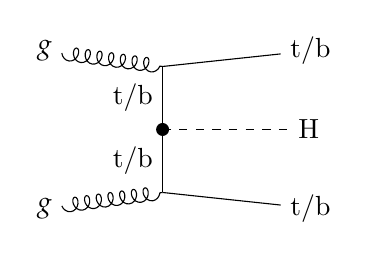
\begin{tikzpicture}[]
    \begin{feynman}
    \vertex (a) {$g$};
    \vertex [right=of a, xshift=0.0cm, yshift=-0.2cm] (b);
    \vertex [right=of b, xshift=0.0cm, yshift=0.2cm] (c) {t/b};

    \vertex [below=of a, xshift=0.0cm, yshift=-0.5cm] (d) {$g$};
    \vertex [right=of d, xshift=0.0cm, yshift=0.2cm] (e);
    \vertex [right=of e, xshift=0.0cm, yshift=-0.2cm] (f) {t/b};

    \vertex [below=of b, xshift=0.0cm, yshift=0.7cm] (cent);

    \vertex [right=of cent, xshift=0.1cm, yshift=-0.0cm] (h) {$\text{H}$};
    \node [dot] at (cent) {};
    \diagram* {
    (a) -- [gluon] (b) -- (c),
    (d) -- [gluon] (e) -- (f),
    (b) -- [edge label'=\({\text{t/b}}\)] (cent) -- [edge label'=\({\text{t/b}}\)] (e),
    (cent) -- [scalar,] (h),
    };
    \end{feynman}
\end{tikzpicture}

\end{document}